\documentclass[11pt, a4paper]{article}
\usepackage[utf8]{inputenc}
\usepackage{amsmath, amssymb}
\usepackage{graphicx}
\usepackage{hyperref}
\usepackage{xcolor}
\usepackage{listings}
\lstset{
    language=Python,
    basicstyle=\ttfamily\small,
    keywordstyle=\color{blue}\bfseries,
    commentstyle=\color{gray}\itshape,
    stringstyle=\color{orange},
    numberstyle=\tiny\color{gray},
    numbers=left,
    stepnumber=1,
    numbersep=8pt,
    frame=single,
    breaklines=true,
    breakatwhitespace=false,
    showstringspaces=false,
    tabsize=4,
    captionpos=b
}
\usepackage{geometry}
\geometry{margin=1in}

\title{EE 325 Digital Signal Processing \\ Assignment 10: Fast Fourier Transform (FFT)}
\author{PERERA J.D.T. \\ E/21/291}
\date{\today}

\begin{document}
\maketitle

\section{1. DFT vs. FFT Complexity}
Let the sequence length be $N = 256$.

\subsection{(a) Direct DFT Computation ($O(N^2)$)}
The direct computation formula is $X[k] = \sum_{n=0}^{N-1} x[n] W_N^{kn}$ where $W_N = e^{-j 2\pi / N}$.
\begin{itemize}
    \item \textbf{Complex Multiplications:} For each $X[k]$, we perform $N$ multiplications. Over $N$ terms, this requires $N^2 = 256^2 = \mathbf{65,536}$ complex multiplications.
    \item \textbf{Complex Additions:} Each $X[k]$ requires the sum of $N$ terms, meaning $(N-1)$ additions. Over $N$ terms: $N(N-1) = 256 \times 255 = \mathbf{65,280}$ complex additions.
\end{itemize}

\subsection{(b) Radix-2 FFT ($O(N \log_2 N)$)}
For a Radix-2 decimation-in-time algorithm:
\begin{itemize}
    \item \textbf{Complex Multiplications:} There are $\log_2 N$ stages, and each stage uses $N/2$ \textit{butterfly} operations. Each butterfly requires only $1$ complex multiplication. Total: $\frac{N}{2} \log_2 N = 128 \times 8 = \mathbf{1,024}$ complex multiplications.
    \item \textbf{Complex Additions:} Each butterfly requires $2$ complex additions. Total: $N \log_2 N = 256 \times 8 = \mathbf{2,048}$ complex additions.
\end{itemize}

\subsection{(c) Ratio of Operations and Savings}
Ratios calculated for $N=256$:
\begin{itemize}
    \item \textbf{Multiplications:} $\frac{N^2}{\frac{N}{2} \log_2 N} = \frac{2N}{\log_2 N} = \frac{512}{8} = \mathbf{64}$
    \item \textbf{Additions:} $\frac{N(N-1)}{N \log_2 N} \approx \frac{N}{\log_2 N} = \frac{256}{8} = \mathbf{32}$
\end{itemize}
The FFT requires roughly a factor of $\mathbf{64}$ fewer multiplications. This demonstrates massive computational savings using the divide-and-conquer approach, enabling scalable real-time processing of longer signals.

\section{2. FFT Combination Formula}
Using a radix-2 DIT FFT, the original $N$-point sequence $x[n]$ is split into an even-indexed subsequence $x_{e}[n] = x[2n]$ and an odd-indexed subsequence $x_{o}[n] = x[2n+1]$, each of length $N/2$. Let their $N/2$-point DFTs be $E[k]$ and $O[k]$. Using the twiddle factor $W_N = e^{-j2\pi/N} $:

\subsection{(a) Expression for $X[k]$}
For the first half of the sequence ($0 \le k < \frac{N}{2}$):
$$ X[k] = E[k] + W_N^k \cdot O[k] $$

\subsection{(b) Expression for $X[k + N/2]$}
For the second half of the sequence ($0 \le k < \frac{N}{2}$):
$$ X[k + N/2] = E[k + N/2] + W_N^{k+N/2} \cdot O[k + N/2] $$
Because both $E[k]$ and $O[k]$ are periodic with period $N/2$ (thus $E[k+N/2] = E[k]$), and $W_N^{k+N/2} = W_N^{N/2} W_N^k = e^{-j\pi} W_N^k = -W_N^k$, this simplifies exactly to:
$$ X[k + N/2] = E[k] - W_N^k \cdot O[k] $$

\subsection{(c) Underpinning the Butterfly Structure}
These two equations construct the fundamental \textbf{butterfly structure} block. To compute \textit{both} $X[k]$ and $X[k+N/2]$, we only need to perform a \textbf{single complex multiplication} ($W_N^k \cdot O[k]$). This single intermediate product is then added to $E[k]$ to form $X[k]$ and subtracted from $E[k]$ to form $X[k+N/2]$. This re-use of multipliers is the direct source of the extreme efficiency and symmetry optimized by the FFT algorithm.

\section{3. Python – Timing DFT and FFT}

A script was created to evaluate a length $N=512$ random complex sequence and compare the timings of a user-defined manual DFT function directly translating the $O(N^2)$ dot product against the optimized `numpy.fft.fft`.

\begin{figure}[h]
    \centering
    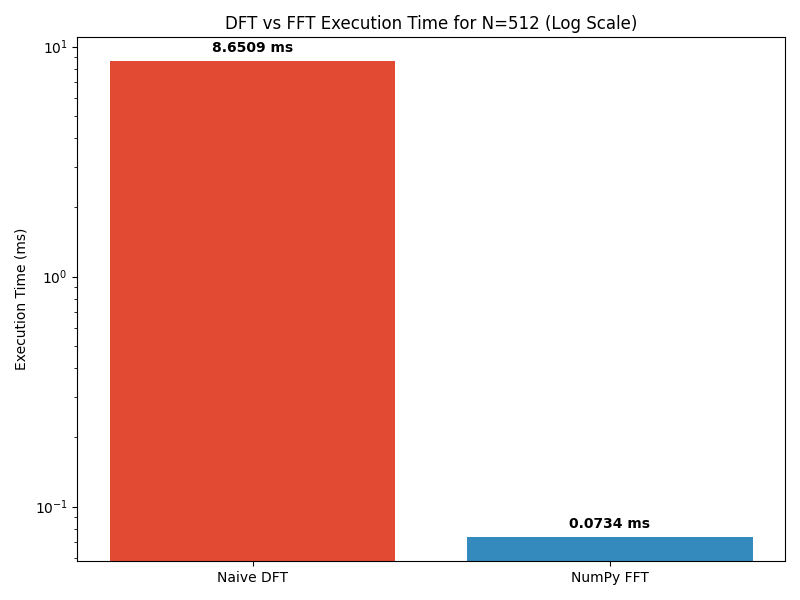
\includegraphics[width=0.8\textwidth]{plots/timing_comparison.png}
    \caption{Empirical Execution Time: Native DFT vs. NumPy FFT}
    \label{fig:timing_comp}
\end{figure}

\subsection{Discussion on Speed-Up Factors}
The theoretical complexity ratio for $N=512$ is approx $\frac{N}{\log_2(N)} = \frac{512}{9} \approx 56.88$.
In practice, the \textit{measured} Python speed-up factor often drastically exceeds $56$x. The empirical differences depend not only on computational complexity but practical execution layers:
\begin{enumerate}
    \item \textbf{Compiled C/Fortran vs. Python Loop Interpreting:} NumPy's `fft` routine calls compiled machine code (C), avoiding interpreter overhead.
    \item \textbf{Memory Footprint:} While `numpy.dot()` is used for the Naive DFT definition, creating the massive $N \times N$ matrix $W_N^{kn}$ explicitly requires $O(N^2)$ memory allocations and reads.
    \item \textbf{Cache Coalescing \& SIMD:} The FFT block algorithms make vastly superior use of CPU level-1 & level-2 cache hierarchy and execute instructions using hardware vectorization optimizations.
\end{enumerate}
This demonstrates that while complexity theories ($\mathcal{O}(N)$ vs $\mathcal{O}(N^2)$) set the expected mathematical scalability rules, true algorithm analysis incorporates memory boundaries and system architecture to dictate realistic speed upgrades.

\appendix
\section{Python Source Code}
\textbf{File:} \texttt{assignment10\_fft\_timing.py}
\begin{lstlisting}[caption={DFT vs. FFT Timing Benchmark -- Assignment 10}]
import numpy as np
import time
import matplotlib.pyplot as plt
import os

def naive_dft(x):
    """Compute DFT of 1D array x using O(N^2) algorithm."""
    N = len(x)
    n = np.arange(N)
    k = n.reshape((N, 1))
    e = np.exp(-2j * np.pi * k * n / N)
    return np.dot(e, x)

def run_timing():
    if not os.path.exists('plots'):
        os.makedirs('plots')

    N = 512
    np.random.seed(42)
    x = np.random.rand(N) + 1j * np.random.rand(N)

    _ = naive_dft(x[:10])
    start_time = time.perf_counter()
    X_dft = naive_dft(x)
    dft_time = time.perf_counter() - start_time

    _ = np.fft.fft(x[:10])
    start_time = time.perf_counter()
    X_fft = np.fft.fft(x)
    fft_time = time.perf_counter() - start_time

    diff = np.max(np.abs(X_dft - X_fft))
    speed_up = dft_time / fft_time if fft_time > 0 else float('inf')
    theoretical_ratio = N / np.log2(N)

    print(f"--- Timing Results for N={N} ---")
    print(f"Naive DFT time: {dft_time*1000:.4f} ms")
    print(f"NumPy FFT time: {fft_time*1000:.4f} ms")
    print(f"Max absolute difference: {diff:.2e}")
    print(f"Measured Speed-up factor (DFT/FFT): {speed_up:.2f}x")
    print(f"Theoretical Ratio (N/log2(N)): {theoretical_ratio:.2f}")

    plt.figure(figsize=(8, 6))
    methods = ['Naive DFT', 'NumPy FFT']
    times = [dft_time * 1000, fft_time * 1000]
    plt.bar(methods, times, color=['#E24A33', '#348ABD'])
    plt.ylabel('Execution Time (ms)')
    plt.yscale('log')
    plt.title(f'DFT vs FFT Execution Time for N={N} (Log Scale)')
    for i, v in enumerate(times):
        plt.text(i, v*1.1, f"{v:.4f} ms", ha='center', fontweight='bold')
    plt.tight_layout()
    output_path = os.path.join('plots', 'timing_comparison.png')
    plt.savefig(output_path)
    print(f"Plot saved to {output_path}")

if __name__ == '__main__':
    run_timing()
\end{lstlisting}

\end{document}
